\documentclass[a4paper,12pt]{article}

% Pakete
\usepackage[utf8]{inputenc}
\usepackage[english]{babel} % Deutsche Sprache
\usepackage{graphicx} % Für Bilder
\usepackage{amsmath} % Für mathematische Formeln
\usepackage{booktabs} % Für Tabellen
\usepackage[hidelinks]{hyperref} % Für Hyperlinks
\usepackage{listings} % Für Code-Blöcke
\usepackage{minted} % Auch für Code-Blöcke
\usepackage{caption}
\usepackage{menukeys}
\usepackage{float}
\usepackage{enumitem}
\usepackage{tocloft}
\usepackage{pgfplots}
\usepackage{pgfplotstable}
\usepgfplotslibrary{groupplots}
\usepackage{siunitx}
\usepackage{multicol}
\usepackage{xcolor}
\usepackage{tikz}
\usepackage{textcomp}
\newcommand{\mytexttilde}{\raisebox{0.5ex}{\texttildelow}}

\usepackage{fancyhdr}
\pagestyle{fancy}

\fancyhf{} % löscht alle aktuellen Kopf- und Fußzeilen

% Kopfzeile: linke Seite = aktuelle Section
\fancyhead[L]{\nouppercase{\leftmark}}

% Fußzeile: linke Seite = Name, rechte Seite = FH Salzburg, zentriert = Seitenzahl
\fancyfoot[L]{Marc Toiflhart, Sebastian Maier}
\fancyfoot[C]{\thepage}
\fancyfoot[R]{Högskolan i Halmstad}

\usepackage{placeins}

\usepackage[
backend=biber,
style=ieee,
sorting=ynt
]{biblatex}

\renewcommand{\listingscaption}{Sourcecode}

\addbibresource{literatur.bib}

\begin{document}

\begin{titlepage}
    \centering
    
\includegraphics[width=5cm]{Resources/hogskolan-halmstad-logo.png} \\[0.5cm] % Logo
    Högskolan i Halmstad \\[0.2cm]
    Biometric Recognition \\[1.5cm]
    
    \hrule
    \vspace{0.4cm} % statt \\[0.4cm]
    {\LARGE \textbf{Laboratory Report}}
    \vspace{0.4cm}
    \hrule
    \vspace{1.5cm} % statt \\[1.5cm]

    {\Large \textbf{Biometric Recognition Laboratory}} \\[0.2cm]
    {\Large Hand Geometry} \\[1cm]
    
    \textbf{Author:} Marc Toiflhart, Sebastian Maier \\[0.2cm]
    \textbf{Date:} \today \\[0.2cm]
    \textbf{Supervisor:} Kevin Hernández Diaz

    \vfill
\end{titlepage}
\newpage

\begin{center}
    \textbf{Summary}
\end{center}

\noindent
This laboratory session focused on the implementation and evaluation of a biometric recognition system based on \textbf{hand geometry}. Individual hand measurements were taken and processed into feature vectors, which were then used to construct a reference vector through averaging and a test vector for verification.

\vspace{0.3em}
\noindent
The system was evaluated in both \textbf{identification mode} (one-to-many comparison) and \textbf{verification mode} (one-to-one comparison) using the Euclidean distance metric. Key performance indicators such as the \emph{rank-based probability function} $P(k)$, the \emph{Cumulative Match Characteristic (CMC)} curve, \emph{False Rejection Rate (FRR)}, \emph{False Acceptance Rate (FAR)}, and the \emph{Equal Error Rate (EER)} were calculated and visualized.

\vspace{0.3em}
\noindent
Threshold values were analyzed to explore the trade-off between \textbf{security} (minimizing FAR) and \textbf{convenience} (minimizing FRR).

\vspace{0.4cm} % statt \\[0.4cm]
\centering
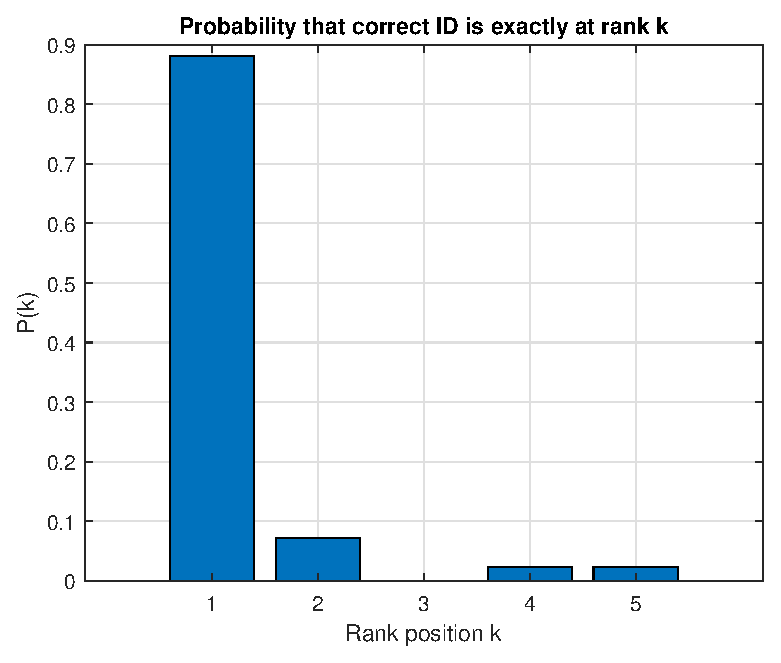
\includegraphics[width=5cm]{Resources/rank_plot.eps} \\[0.5cm]

% Inhaltsverzeichnis
\tableofcontents
\newpage

% Abbildungsverzeichnis
\listoffigures
\newpage

% Tabellenverzeichnis
\listoftables
\newpage


\newpage
\printbibliography

\end{document}